\documentclass[UTF8]{ctexart}
\usepackage{amsmath}
\usepackage{amssymb}
\usepackage{booktabs}
\usepackage{background}
\usepackage{caption,subcaption}
\usepackage{CJKfntef}
\usepackage{cprotect}
\usepackage{enumitem}
\usepackage{fancyhdr}
\usepackage{float}
\usepackage{fontspec}
%\usepackage{fourier}
\usepackage{geometry}
\usepackage{listings}
\usepackage{tcolorbox}
\usepackage{tikz}
\usetikzlibrary{arrows.meta}
\usepackage{xcolor}

\geometry{a5paper, top=0.1cm, left=1cm, right=1cm, bottom=1cm, footskip=0.1cm}
\setCJKmainfont[BoldFont={汉仪文黑-85W},ItalicFont={方正苏新诗柳楷简体}]{汉仪文黑-55W}
\setfontfamily\Issue{Century Schoolbook}
\setfontfamily\Genshin{Genshin Teyvat Lingua Franca}
\newCJKfontfamily\TitleFont{思源宋体 CN Heavy}
\newfontfamily\timesnewroman{Times New Roman}
%\reversemarginpar

\pagestyle{fancy}
\fancyhf{}
\cfoot{\sffamily\footnotesize{-\ \thepage\ -}}
%\CTEXsetup[format = {\centering\bfseries\large}, beforeskip = 3pt, afterskip = 3pt]{section}

\colorlet{darkcyan}{cyan!50!black}
\newcommand\Black[1]{\textcolor[gray]{0.3}{#1}}
\newcommand\Brown[1]{\textcolor[HTML]{998A4E}{#1}}
\newcommand\Emph[1]{\colorbox{green!10}{\textcolor{green!30!black}{#1}}}
\newcommand\Notes[1]{\textcolor{yellow!50!black}{\small #1}}
\newcommand\Example[1]{\textcolor{cyan!70!black}{\small #1}}
\newcommand\keyword[1]{\textcolor{violet}{\textbf{\texttt{#1}}}}

\newtcolorbox{mybox}[1][其他规则]{colback=cyan!10, colframe=cyan, arc=1pt, title={#1}}

\renewcommand\d{\mathrm{d}}

\lstset{
    basicstyle=\small\ttfamily, %注意行末有逗号!
    keywordstyle=\bfseries\color{blue!70!black},
    commentstyle=\color{cyan!90!black},
    stringstyle=\color{green!40!black},
    columns=flexible,
    numbers=left,
    numberstyle=\footnotesize,
    escapechar=`,
    frame=shadowbox,
    %rulesepcolor=\color{red!20!blue!20!green!20}
    backgroundcolor=\color{cyan!5!white},
    language = Java,
    tabsize = 4,
    breaklines = true,
}

\newcommand\IssueNumber{31}
\newcommand\Date{2024-6-16}
%\newcommand\Contributer{@金光日}
\newcommand\Subject{高级程序设计语言(C++)}


\begin{document}
\backgroundsetup{contents=
\includegraphics{上半示例.png}, center, scale=1, angle=0, opacity=1}
\BgThispage
\begin{center}
%{\scriptsize\Issue \textcolor[HTML]{C8BA83}{\Genshin WEEKLY TIPS}}
\phantom{...}

{\Large\textcolor{brown!40!white}{\makebox[10cm][s]{\Genshin WEEKLY KNOWLEDGE TIPS}}}

\vspace{-2em}

{\Huge\bfseries\TitleFont \Black{知\ 识\ 小\ 料}}


\vspace{-0.1cm}
{\footnotesize \Brown{「电计 2203 班」周常规知识整理共享}}
\end{center}

\vspace{-0.5cm}


\begin{figure}[H]
\hspace{1cm}
\begin{minipage}[t]{0.3\textwidth}
\centering
    \Brown{\Genshin ISSUE}

    \vspace{-0.6cm}
    \Huge \Issue\slshape\bfseries\Black{\IssueNumber}
\end{minipage}
\hfill
\begin{minipage}[t]{0.35\textwidth}
\centering
    \Brown{日期:\Date} \\
%\vspace{-0.1cm}
%    \Brown{贡献者:\Contributer} \\
\vspace{-0.1cm}
    \Brown{学科:\Subject} \\
\end{minipage}
\hspace{0.8cm}
\end{figure}

{\color{cyan!50!black}
C++ 考试选手应知应会的 Java 知识。
}

\section{Java语言概述}

\begin{table}[htb]
  \centering
  \begin{tabular}{ccc}
  \toprule
    & Java & C++ \\
  \midrule
  开发方法 & 纯面向对象 & 面向对象 \\
  执行原理 & 解释型语言 & 编译型语言 \\
  有无指针 & 无 & 有 \\
  异常处理 & 出色 & 一般 \\
  执行效率 & 较慢 & 较快 \\
  \bottomrule
  \end{tabular}
  \caption{Java 与 C++ 的主要对比}\label{tab:java-and-c++}
\end{table}

结构化程序设计方法的主要原则:自顶向下、逐步求精、模块化。

\paragraph{JVM,JRE,JDK名词辨析}

\begin{itemize}[itemsep=0pt,parsep=0pt]
  \item \Emph{JVM}(Java虚拟机)——是Java语言运行的虚拟机;
  \item \Emph{JRE}(包含JVM和核心库)——是Java语言运行的环境;
  \item \Emph{JDK}(包含JRE和开发工具)——是Java开发人员使用的工具;
  \item 总结起来,\underline{JDK包含JRE,JRE包含JVM}。
\end{itemize}

\paragraph{Java程序的执行流程}

\begin{itemize}[itemsep=0pt,parsep=0pt]
  \item \Emph{编写程序}——程序员编写代码,得到源文件,目标为 \Emph{.java文件};
  \item \Emph{编译文件}——用编译器编译源文件,得到字节码文件,目标为 \Emph{.class 文件};
  \item \Emph{解释文件}——用 JVM(Java虚拟机)解释字节码文件,得到结果。
\end{itemize}

\newpage
\backgroundsetup{contents=
\includegraphics{空白示例.png}, center, scale=1, angle=0, opacity=1}
\BgThispage
\paragraph{Java标识符——类名、变量名}

\begin{itemize}[itemsep=0pt,parsep=0pt]
  \item \textbf{允许}——字母、数字、下划线(\verb!_!)、美元(\verb!$!)组成
  \item \textbf{不允许}——数字开头
  \item \textbf{不允许}——包含 \verb!@!、\verb!#! 等特殊字符和空格
  \item \textbf{不允许}——与各种关键字重名
\end{itemize}

原则上类名以大写字母开头,对象名、函数名以小写字母开头。

示例:变量名如 \verb!a_b$c!、\verb!a1! 正确;如 \verb!a_b@c!、\verb!1a!、\textbf{\texttt{goto}} \footnote{其实Java语言中有 \keyword{goto} 这个关键字,但是这个指令不允许使用。}错误。

关键字举例:
\begin{itemize}[itemsep=0pt,parsep=0pt]
  \item \keyword{true}、\keyword{false}——小写才是关键字
  \item \keyword{implements}、\keyword{extends}——用于类的继承和接口调用
  \item \keyword{var}、\keyword{null}——C++没有而Java特有的
\end{itemize}

\section{类与对象·基本}
\begin{center}
  \Emph{类}是对象的抽象化,\Emph{对象}是类的具体化,\Emph{实例}是对象的别名。
\end{center}

\subsection{类的基本定义}
类的基本定义格式:(成员变量 + 构造器 + 方法)
\begin{lstlisting}
public class Person {
    String name; //类的成员变量
    int age;
    Person(String name, int age){ //构造器
        this.name = name;
        this.age = age;
    }
    void say(String content){  //类的方法
        System.out.println(content);
    }
}
\end{lstlisting}

\subsection{构造器}
构造器就是一种特殊的方法,用于创建对象。比如上面例子的
\begin{quote}
  \verb!Person(String name, int age)!
\end{quote}
就是构造器。

在主方法\footnote{在Java中,「函数」一般称作「方法」。}中,可以使用 \verb!Person p = new Person("XiaoMing", 19);! 这样的语句来构造一个对象 $p$。

\begin{mybox}
\begin{itemize}[itemsep=0pt,parsep=0pt]
  \item 构造器名须与类名相同。
  \item 构造器名不要指定返回值。
  \item 如果没有指定构造器,则系统会默认提供一个空的构造器。
\end{itemize}
\end{mybox}

\subsection{对象访问与 \keyword{this} 的使用}
对于上述的 $p$ 对象,可以用点号操作符来访问它的成员变量与方法。

\begin{quote}
  \verb!p.age = 20;! 或者 \verb!p.say("Hello");!
\end{quote}

在构造器中,\keyword{this} 总是指向调用该方法的对象。比如刚刚的例子,构造器中的 \keyword{this} 指向的就是 $p$,构造的过程即表示把 $p$ 的成员变量 \verb!p.name! 赋值为 \verb!name!,把另一个成员变量 \verb!p.age! 赋值为 \verb!age!。

\subsection{变量}
\begin{figure}[htb]
  \centering
  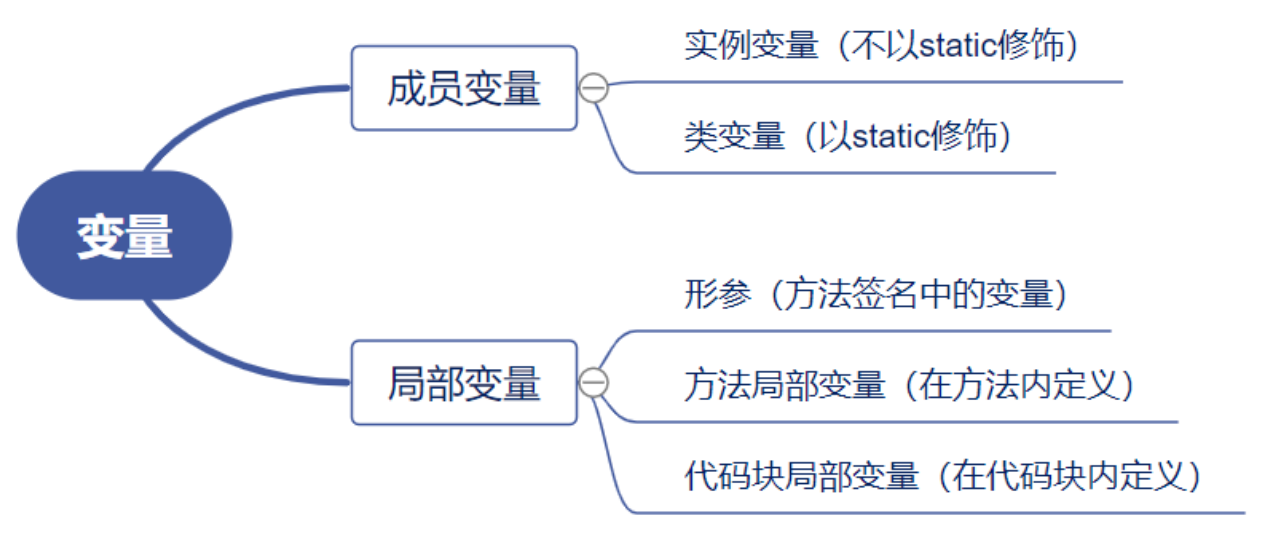
\includegraphics[width=10cm]{变量.png}
  \caption{变量分类图}\label{fig:variable}
\end{figure}

用一个例子捋清楚这些变量:
\begin{lstlisting}
public class Person{
    String name;    //成员变量·实例变量
    static int age; //成员变量·类变量
    Person(String newName, int newAge){ //局部变量·形参
        this.name = newName;
        {
            int x = 1;  //局部变量·方法局部(也是代码块局部)
            this.age = newAge + 1;
        }
    }
}
\end{lstlisting}

\begin{mybox}
\begin{enumerate}[itemsep=0pt,parsep=0pt]
  \item 对于成员变量,以下的访问是允许的:
  \begin{itemize}[itemsep=0pt,parsep=0pt]
    \item \verb!实例.实例变量!——\verb!p.name!
    \item \verb!实例.类变量!——\verb!p.age!
    \item \verb!类.类变量!——\verb!Person.age!
  \end{itemize}
  \item 对于成员变量,初始值是系统会默认分配的。对于局部变量,必须明确初始化。
  \item 类变量的作用域是整个类,实例变量的作用域仅限于其实例。
\end{enumerate}
\end{mybox}

\begin{figure}[htb]
  \centering
  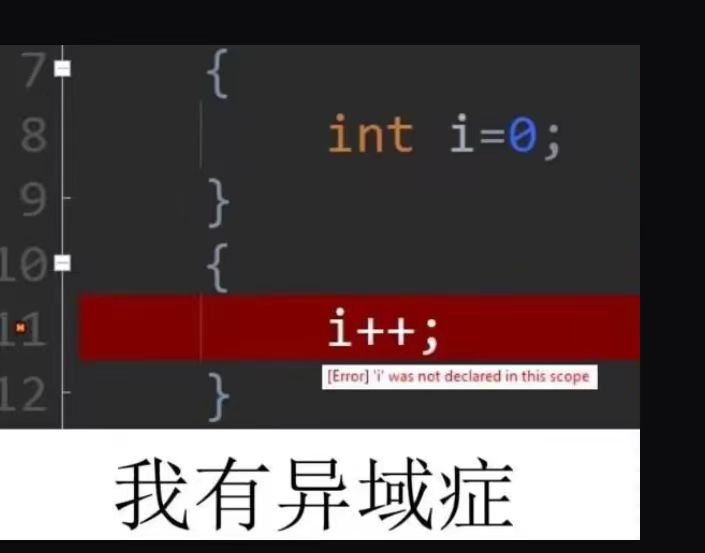
\includegraphics[width=5cm]{代码块局部变量.jpg}
  \caption{代码块局部变量在离开其作用域后立即销毁}\label{fig:codeBlockVar}
\end{figure}

\subsection{方法}

\begin{itemize}[itemsep=0pt,parsep=0pt]
  \item 未使用 \keyword{static} 修饰的方法只能拿实例调用,不能拿类调用。
  \item 使用了 \keyword{static} 修饰的方法既能拿实例调用,也能拿类调用。
\end{itemize}

\begin{lstlisting}
class Person{
    //成员变量与构造器的定义省略
    public void sing() { ... } //无static,只能实例调用
    public static void run() { ... } //有static,实例和类都能调用
}
public class Test{
    public static void main(String [] args){
        Person p = new Person("小明",19);
        p.sing();     //实例调用
        p.run();      //实例调用
        Person.run(); //类调用
    }
}
\end{lstlisting}

\section{类与对象·封装、继承、多态}
封装、继承、多态,即是面向对象的三个特征。

\subsection{封装}
封装是一种将抽象性接口细节包装、隐藏起来的方式。通过访问控制符,可以增加程序安全性。

访问控制符:\keyword{public} > \keyword{protected} > \keyword{default} > \keyword{private}

比如说,\keyword{public} 修饰的方法、变量可以在全局范围内访问,\keyword{private}修饰的方法、变量仅限于类内访问。下列的例子中,要修改对象 $p$ 的信息,不可以直接访问 \keyword{private} 修饰的 \verb!p.name! 和 \verb!p.age!,而是可以用 \keyword{public} 修饰的方法 \verb!setInformation! 来实现。
\begin{lstlisting}
class Person{
    private String name; //私有的成员变量
    private int age;
    public Person(String name, int age){ //公有的构造器
        this.name = name;
        this.age = age;
    }
    public void setInformation(String name, int age){ //公有的方法
        this.name = name;
        this.age = age;
    }
}
public class Test{
    public static void main(String [] args){
        Person p = new Person("小明", 19); //构造器是public的,所以在Person类外可以使用
//      p.age = 20; //这两个成员变量都是private的,不可以类外访问,所以会出错
//      p.name = "小红";
        p.setInformation("小红", 20); //这个方法是public的,可以类外访问
    }
}
\end{lstlisting}

\subsection{继承}

Java 也有继承的操作,不过\Emph{一个类至多只能继承一个父类},即不支持多继承。

子类 Son 继承父类 Father 的变量 x,同时也有其新的变量 y。子类能够拥有父类全部的属性、方法(除非是 \keyword{private})。

\begin{lstlisting}
class Father{ //父类的定义
    int x;
    Father(int newX){
        this.x = newX;
    }
}
class Son extends Father{ //子类的定义
    int y;
    Son(int newX, int newY){
        super(newX); //super关键字用于调用父类的构造器(方法、属性等)
        this.y = newY;
    }
}
\end{lstlisting}


\subsection{多态}
在 C++ 中,多态性主要体现为函数与运算符的重载。在 Java 中,多态性则主要体现为函数的重载(Overload)与重写(Override)。

\begin{itemize}[itemsep=0pt,parsep=0pt]
  \item 重载(Overload)——多个同名但是形参列表不同的方法,就是方法重载。
  \item 重写(Override)——用子类的某个方法覆盖父类的同名方法,就是方法重写。
\end{itemize}

比如,以下的例子实现了构造器的重载。(类似于C++的构造函数和「拷贝构造函数」的关系)
\begin{lstlisting}
class Person{
    String name;
    int age;
    Person(String name, int age){ //带String,int类的两个参数的构造器
        this.name = name;
        this.age = age;
    }
    Person(Person p){ //带Person类的一个参数的构造器
        this.name = p.name;
        this.age = p.age;
    }
}
\end{lstlisting}

再比如,以下的例子实现了run方法的重写。
\begin{lstlisting}
class Animal{
    void run() { System.out.println("动物的run方法"); }
}
class Dog extends Animal{
    void run() { System.out.println("狗狗的run方法"); }
}
public class Test{
    public static void main(String [] args){
        Dog d = new Dog();
        d.run();   //执行狗狗的run方法,该方法重写了父类动物的run方法
    }
}
\end{lstlisting}

\section{类与对象·特殊的类}
\subsection{单例类}
如果一个类始终只能创建一个对象,那就是单例类。

\subsection{终稿类}
如果一个类不能被继承,那就是终稿类。用\keyword{final}修饰。

典型的终稿类是 \texttt{String} 类。

终稿变量(\keyword{final} 修饰的变量)是一经初始化就不可修改的变量。

\subsection{抽象类}
如果一个类不能直接创建对象(不能被实例化),那就是抽象类。用\keyword{abstract}修饰。

这种类存在的意义在于提供一个模板,用子类继承抽象类,从而实现各种具体的功能。

如果一个类含有抽象方法,那整个类都必须用\keyword{abstract}修饰。

\subsection{接口}
接口是抽象类的一种,用\keyword{interface} 来定义接口,用 \keyword{implements}来调用接口。

一个类可以实现多个接口,这使得Java克服了不能多继承的困难。

\subsection{内部类}
把一个类放在另一个类的内部进行定义,那就是内部类。

如果把一个类放在某个方法的内部进行定义,那就是局部内部类。

\subsection{Java 的垃圾回收机制}
当对象永久性地失去引用时,系统就会回收其所占的资源。而在回收任何对象之前,总会先调用它的 \verb!finalize! 方法以试图「救活」它,如果能「救活」则该对象继续运行,如果「救不活」那就只能回收资源了。

\newpage
\backgroundsetup{contents=
\includegraphics{下半示例.png}, center, scale=1, angle=0, opacity=1}
\BgThispage
\subsection{交付包(.jar)}
Java归档文件(JAR)是将若干个 \verb!.class! 文件压缩、归档并交付给用户使用的交付包,扩展名为 \verb!.jar!。

.jar 文件装的是 .class 文件,可以用压缩软件来解压缩。

\end{document} 